\documentclass[12pt]{diazessay}

\usepackage{bashful}
\usepackage{hyperref}

%----------------------------------------------------------------------------------------
%	Comment this out if you do not have `texcount` installed on your $PATH
%----------------------------------------------------------------------------------------
%\bash
%command -v texcount &> /dev/null && texcount -sum -1 csci-724-paper.tex
%\END

%Shorthand formatting commands
\newcommand{\F}[1]{$\quad$\texttt{#1}}
\newcommand{\A}{$\alpha$}
\newcommand{\B}{$\beta$}
\newcommand{\Bool   }{\texttt{Bool}}
\newcommand{\Nat    }{\texttt{Natural}}
\newcommand{\Integer}{\texttt{Integer}}
\newcommand{\Double }{\texttt{Double}}
\newcommand{\List   }{\texttt{List}}
\newcommand{\Type   }{\texttt{Type}}

%----------------------------------------------------------------------------------------
%	TITLE SECTION
%----------------------------------------------------------------------------------------

\title{\texttt{\huge{An analysis about effectiveness\\\vspace{-3mm}of structure-aware fuzzing} \\\vspace{-0.35cm} {\large A Hunter College CSCI-795 Project Proposal}\\\normalsize\url{https://github.com/recursion-ninja/Superion-YAML}}} % Title and subtitle

\author{\texttt{{\Huge Team:}\\\vspace*{-0.5em} 
		Sabina Bhuiyan \\\vspace*{-0.5em} 
		Kyoungwoo Lee \\\vspace*{-0.5em}
		Chuanyao Lin \\\vspace*{-0.25em}
		Alex Washburn}} % Author and institution

\date{\texttt{\today}} % Date, use \date{} for no date

\pagestyle{empty}
%----------------------------------------------------------------------------------------

\begin{document}

\maketitle % Print the title section

\vspace{2cm}
\section*{Abstract}

%%%%%%%%%%%%%%%%%%%%%%%%%%%%%%%%%%%%%
%   NO citations in the abstract!   %
%%%%%%%%%%%%%%%%%%%%%%%%%%%%%%%%%%%%%

For our project, we propose exploring the efficiency of grey-box fuzzing programs with structured inputs compared to generically mutated random-like inputs.
The assessment will be adapted to test three major file formats: YAML, JSON, and Markdown.
Of all the ubiquitous file formats, these three are currently the most popular that both, are consumed as input by a wide array of programs, and have enough CVEs that we can gauge the efficacy with.

There are some state-of-the-art fuzzers that accentuate their effectiveness with structured input such as Gramatron, Superion, and Mayhem.
We take Gramatron and Superion as extension targets that can generate our test file formats, as they are both open sources but Mayhem is not.
Grimoire is a fuzzer that, without structured inputs, can perform grammar awareness fuzzing by itself.

In the course of this project, we will extend the functionality of these two fuzzers and scrutinize the fuzzing capabilities of these extensions compared to Grimoire against a corpus of CVEs of our three target file formats.
Our comparative metric will be both qualitative and quantitative; measuring coverage of CVEs and execution time to obtain coverage.

\clearpage
\section*{Introduction}
Fuzzing is a venerable application security testing technique developed in the late '80s\cite{Barton1988} and published in 1990\cite{Miller1990}.
Fuzzing tools generate input which is directed towards the program under test and detect if the input was accepted or caused unexpected behavior.
Unexpected behavior can take many forms, such as infinite loops, stack smashing, buffer overflows, arithmetic overflows or errors, and illegal program states.
Fuzzing tools themselves can take many forms\cite{ModelBasedFuzzing}\cite{GrammarBasedFuzzing}\cite{ProtocolBasedFuzzing} and modify program input in many ways.
Different fuzzing tools tend to specialize in a few related forms of input\cite{InputDiversity} manipulation.
There are three main classes of interaction between the fuzzer and the program under test, black-box\cite{takanen2018fuzzing}, grey-box, and white-box\cite{fuzzingsurvey}.
In a black-box scenario, the fuzzer has no knowledge of the program's internal structure and cannot use any program-specific information to direct its fuzzing efforts.
In a grey-box scenario, the fuzzer gleans information from its previous input to guide future inputs.
Lastly, in a white-box scenario, the fuzzer can utilize program analysis to inform its fuzzing inputs.

There are also two broad classes of inputs fuzzers generate; naive and structured\cite{fuzzingsurvey}.
Naive inputs do not provide any guarantees regarding its form.
Structured inputs, on the other hand, can be defined to always preserve desired structures within the inputs.

AFL\cite{AFL_page} is one of the best-known fuzzing tools. AFL relies on genetic algorithm techniques\cite{InputMutationAlgorithm} to mutate acceptable input into an input that triggers unexpected behavior.
Using the generic AFL approach, inputs would be mutated randomly, and an initially valid structured input would quickly become invalid.
The invalid input in this scenario, is not the one that introduces the vulnerability of the target system.
Random inputs just fail to run the major part of the target system, suspended by the type checkers or the input validators.
This is a longstanding problem in the art of fuzzing and is the subject of emerging research.
Generating consistently well-structured inputs\cite{structuredInput} via "grammar-aware" mutations is one such technique for addressing the problem of randomly mutated inputs.
AFL is a poster child for efficient, naive input fuzzing.

\section*{Motivation}
We are aware of the topic "Going Beyond Coverage-Guided Fuzzing with Structured Fuzzing" by Jonathan Metzman in the Black Hat USA 2019\cite{blackhat2019}.
In the talk, the speaker presented structured fuzzing and how to improve the fuzzer by adding structure awareness to it. 
Therefore, we started our project with learning “What is Structured Fuzzing?”, and the concept of writing the well-structured inputs via "grammar-aware" mutations to improve the fuzzers we chose.


Superion\cite{superion} is an fairly recent open source fuzzing tool created by modifying and extending AFL to produce structured inputs released in 2018.
Superion currently generates valid JavaScript and XML inputs by taking a context free grammar and an input seed, then performing a series of "grammar-aware" mutations to create a sequence of validly structured inputs.
The results of Superion show a great increase in fuzzing efficacy when targeting programs which expect structured input.

\begin{center}
    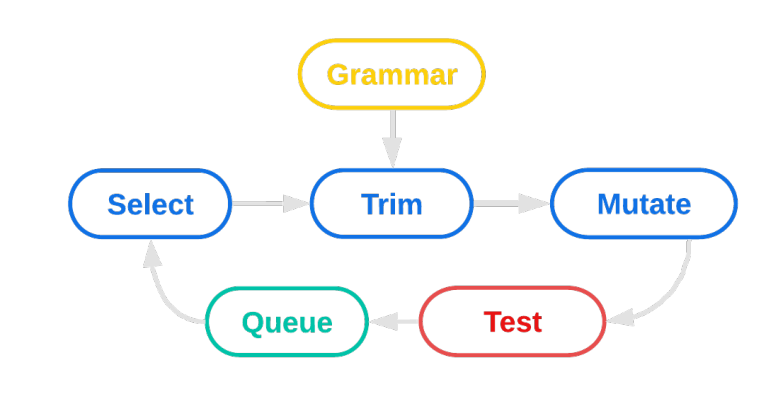
\includegraphics[scale=0.4]{superionfig.jpg}
\end{center}

Gramatron\cite{srivastava2021gramatron} is a second, and even more recent, open source fuzzing tool designed to produce structured inputs.
Released in 2021, Gramatron was designed with new mutation algorithms to increase the speed at which defects are discovered.
It does this by reducing the number of mutation steps from the input seed to the trigger input, rather than simply optimizing the speed at which new inputs can be generated.
Gramatron currently generates structured PHP and JavaScript as inputs.

Grimoire\cite{GRIMOIRE} is a structured input fuzzer which does not require an explicit structural definition to effectively generate fuzzing inputs.
Instead, Grimoire deduces the required input structure via feedback from the program.
Initial research suggests that this form of structure-inferring fuzz technique may be more effective than explicitly defined structured input fuzzing as Grimoire can probe corner cases which are excluded from formal grammars.

We propose extending the capabilities of Gramatron and Superion to support generating three structured inputs: YAML\cite{YAMLdraft}, JSON and Markdown.
We will compare the efficacy of our extended versions of Gramatron and Superion to both Grimoire and previous work targeted at fuzzing these three file formats.

Aside from the fact that there is room for these formats on extending our target fuzzers, we have numerous reasons for selecting YAML, JSON, and Markdown as our extension language.
First, it has a well-defined formal grammar, allowing it to be quickly and reliably integrated into the two fuzzers.
Second, these file formats are ubiquitous input formats.
This ubiquity makes our target languages a well-motivated language to extend these fuzzers to support.
Lastly, to a proper assessment of its performances, languages that have a sufficient corpus of CVEs are required. 
These languages have a decent amount CVEs that we can work with.
There are 108(YAML), 664(JSON), and 103(Markdown) CVEs on MITRE\cite{MITRE}.

The goal of this project is to extend the capabilities of both Gramatron and Superion, then compare their performance along with Grimoire towards replicated selected CVEs.
If the novel defect(s) are discovered and notable, we will consider the ancillary goal of publishing new CVE(s).

By utilizing the three fuzzers- Gramatron, Superion, and Grimoire- we hope to draw a rich comparison of modern fuzzing techniques.
After taking the cybersecurity course and learning about the fuzzing software, we hope to be well-equipped in determining whether these tools might be utilized as an automated method of finding software exploits in other domains.

Although we have confined our extension targets to two cutting-edge fuzzers for various reasons, 
there are other modern fuzzers that can be tackled in future projects such as; CodeAlchemist\cite{CodeAlchemist1}\cite{CodeAlchemist2}, Hawkeye\cite{Hawkeye}, Angora\cite{Angora1}\cite{Angora2}, CollAFL\cite{CollAFL}, IoTFuzzer\cite{IoTFuzzer}, RedQueen\,\cite{redqueen}, Nautilus\,\cite{Nautilus1}\cite{Nautilus2}, Periscope\cite{PeriScope1}\cite{PeriScope2}, T-Fuzz\,\cite{TFuzz1}\cite{TFuzz2}, Chopper\cite{Chopper}, QSYM\cite{QSYM1}\cite{QSYM2}, DigFuzz\cite{DigFuzz}, and FairFuzz\cite{FairFuzz1}\cite{FairFuzz2}.
All these tools are distinguished in their specialized scoped, but we have decided to work with Gramatron and Superion as these are open-sourced projects, and are specialized in generating structured inputs in a modular manner.


% \clearpage


\section*{Approach}

We will extend the functionality of Gramatron to generate mutable, structure-aware YAML, JSON, and Markdown output.
Additionally, we will extend the functionality of Superion to generate mutable, structure-aware outputs in the same three target languages.
Both projects are open source and are modular in their design for incorporating new grammars.
These extensions, which are valuable to the wider fuzzing community, ought not to be too onerous.

Qualitatively, we will compose a corpus of CVEs discovered from previous work.
There are currently over 100 CVEs cataloged on MITRE\cite{MITRE} for each of our target languages.
We will select a reproducible subset of these CVEs to use as our coverage test.
The degree to which our extended fuzzing programs discover the known CVEs will be our qualitative metric of completeness.

Quantitatively, we will measure the execution time of each extended fuzzing program.
We will perform a comparison between Gramatron, Superion, and Grimoire mutation strategies in terms of how quickly they discover the known CVEs.
Where possible, we will also compare the performance of Gramatron, Superion, and Grimoire to previously published work which provides execution metrics.

We will generate a series of ``seed inputs'' for our three fuzzers which are accepted by the programs under test and generate expected behavior.
We will then allow these fuzzing programs to mutate the seed inputs\cite{Seed} according to their unique internal algorithms in order to probe for the CVE defects.
During the initial calibration of the fuzzers, we will manually monitor progress and adapt the seeds as needed to ensure that they are effectively probing the target programs.
Our programs under test will be those cataloged from the selected CVEs corpus.

The process of comparing these fuzzers opens the possibility of discovering novel defects outside the pre-selected CVEs.
While investigating these novel defects are outside the scope of this course project, we will take care to preserve the triggering inputs for future work.

The team expects to use their personal, commodity computer hardware to carry out this project.
However, should hardware constraints be discovered or it is determined to be beneficial for the project, the team members will have access to the DETER computing cluster at Hunter College.
Additionally, we can attempt to use Hunter's research credits on AWS.
Either way, we hope to reach a point of automation in the project where parallelization on a cluster is achievable, but can cope with commodity hardware.

Our project quantifying and qualifying the performance of these three modern fuzzers will lend valuable insight into the efficacy between these programs' internal algorithms, and how they compare to previous work.
This is of academic interest as it will inform the direction of future fuzzing research.


\section*{Preliminary Results}
\label{results}
\vspace{-0.25cm}

For each target language, we have selected 10 CVEs to administer qualitative evaluation of our extended fuzzers.
The table below is a corpus of CVEs that we choose to run our tests on.
These are some of the most recent known defects on open-sourced applications with reference to our target languages.

\begin{table}[h!] \centering \scalebox{1} { \begin{tabular}{V{4}l|l|lV{4}} \hlineB{3}
	\multicolumn{1}{V{4}c|}{YAML} & \multicolumn{1}{c|}{JSON} & \multicolumn{1}{cV{4}}{Markdown}  \\ \hline
	\texttt{CVE-2021-42139\cite{CVE-2021-42139}} & \texttt{CVE-2021-41106\cite{CVE-2021-41106}} & \texttt{CVE-2021-39887\cite{CVE-2021-39887}} \\ \hline
	\texttt{CVE-2021-39194\cite{CVE-2021-39194}} & \texttt{CVE-2021-39215\cite{CVE-2021-39215}} & \texttt{CVE-2021-39199\cite{CVE-2021-39199}} \\ \hline
	\texttt{CVE-2021-39132\cite{CVE-2021-39132}} & \texttt{CVE-2021-39205\cite{CVE-2021-39205}} & \texttt{CVE-2021-39175\cite{CVE-2021-39175}} \\ \hline
	\texttt{CVE-2021-36793\cite{CVE-2021-36793}} & \texttt{CVE-2021-32781\cite{CVE-2021-32781}} & \texttt{CVE-2021-37700\cite{CVE-2021-37700}} \\ \hline
	\texttt{CVE-2021-36162\cite{CVE-2021-36162}} & \texttt{CVE-2021-32677\cite{CVE-2021-32677}} & \texttt{CVE-2021-29503\cite{CVE-2021-29503}} \\ \hline
	\texttt{CVE-2021-30180\cite{CVE-2021-30180}} & \texttt{CVE-2021-31618\cite{CVE-2021-31618}} & \texttt{CVE-2021-29475\cite{CVE-2021-29475}} \\ \hline
	\texttt{CVE-2021-22557\cite{CVE-2021-22557}} & \texttt{CVE-2021-30641\cite{CVE-2021-30641}} & \texttt{CVE-2021-29474\cite{CVE-2021-29474}} \\ \hline
	\texttt{CVE-2021-21250\cite{CVE-2021-21250}} & \texttt{CVE-2021-30179\cite{CVE-2021-30179}} & \texttt{CVE-2021-27907\cite{CVE-2021-27907}} \\ \hline
	\texttt{CVE-2021-21249\cite{CVE-2021-21249}} & \texttt{CVE-2021-26691\cite{CVE-2021-26691}} & \texttt{CVE-2021-27578\cite{CVE-2021-27578}} \\ \hline
	\texttt{CVE-2020-7729\cite{CVE-2020-7729}} & \texttt{CVE-2021-26690\cite{CVE-2021-26690}} & \texttt{CVE-2021-22242\cite{CVE-2021-22242}} \\ \hlineB{3}
\end{tabular}  } 
\vspace{3mm}\\ \textbf{Table 1.} Target CVEs for each languages
\end{table}

We have administered two major tasks prior to extending the functionality of each fuzzers.
First, we have set up Gramatron and Superion to run in the test environment.
The input generators for each fuzzer successfully constructed seed files\cite{superion-example}\cite{gramatron-example}that conform to the grammatic constraints of Javascript.
Configuring grammar-specific protocols and rules for each fuzzer was followed by the environment setup.
This was done through the course of literature review and presentation preparation, and we have built the JSON grammar definition file\cite{json-source.json} for extending Gramatron.

\vspace{6mm}
\hrule height 0.4mm
\begingroup \fontsize{12pt}{12pt} \selectfont \begin{alltt}
\input{input.js}
\end{alltt} \vspace{-6mm} \endgroup \hrule height 0.4mm
\vspace{3mm}
\centerline{\textbf{Figure 1.} Input created from Grammar-aware input generators}


\section*{Discussion}
Based on the fuzzing tests conducted on the selected CVEs, we found that our extension of Superion and Gramatron were feasible. 

Superion generated an input that resembled human-written javascript, by taking a context free grammar and an input seed, then performing a series of "grammar-aware" mutations to create a sequence of validly structured inputs. Superion created an input that was similar to what we were looking for. 

Meanwhile, Gramatron was harder to read. This may be because Gramatron reduces the number of mutation steps from the input seed to the trigger input. 

We hope to show that our tests on the extensions of Superion and Gramatron will be more performant than those conducted on Grimoire since Superion and Gramatron directly produce the inputs, while Grimoire creates the input from feedback, rather than a defined structure.

\section*{Future Experimentation}
For the future work, Grimoire, Gramatron, Superion could be combined for large-scale testing to explore the new CVEs. 
We can combine the structured inputs generated from Gramatron, Superion with Grimoire, since Grimoire generates input only based on the feedback.
Lastly, we can keep extending the fuzzers to support more languages for generating the grammar aware inputs.

\section*{Division of Labor}

Alex Washburn devised the main concept of the project.
Alex Washburn and Chuanyao Lin designed the project and derive fuzzing techniques.
Sabina Bhuiyan and Kyoungwoo Lee conducted literature reviews and related research on extending the fuzzing tools.
Chuanyao Lin and Kyoungwoo Lee extended Gramatron to support targeted file formats.
Alex Washburn and Sabina Bhuiyan extended Superion to support targeted languages.
Kyoungwoo Lee and Alex Washburn configured the fuzzing environment on AWS/DETER.
Each member conducted fuzzing on the divided set of CVEs.
Chuanyao Lin and Sabina Bhuiyan analyzed the project in comparison with Grimoire and authored the reports.


\clearpage
\section*{Timeline}

The project timeline is partially defined by the course syllabus where deadlines are concerned and partially team defined where the syllabus does not give guidance.
The team has collaboratively discussed and drafted a tentative timeline of the project based on our assumptions of progress and integrated this with the deliverable deadlines laid out in the course syllabus. The current, tentative project timeline is as follows:

\begin{enumerate}[label={}]
	\item \texttt{2021-08-29:} Form team and brainstorm project ideas
	\item \texttt{2021-09-05:} \textbf{Project Proposal due}
	\item \texttt{2021-09-12:} Revise and resubmit proposal
	\item \texttt{2021-09-19:} Background research \& Revise \/ resubmit proposal
	\item \texttt{2021-09-26:} Begin modifying Superion \& Gramatron to generate YAML, JSON, and Markdown
	\item \texttt{2021-10-03:} Finilize proposal, Complete modified Gramatron \& Superion generating , Collect and finalize CVEs corpus
	\item \texttt{2021-10-10:} \textbf{Midterm project presentations due} \hfill (Show fuzzing YAML output)
	\item \texttt{2021-10-17:} \textbf{Midterm project reports due} \hfill (Tune fuzzing instrumentation)
	\item \texttt{2021-10-24:} Tune 3 fuzzers instrumentation with programs under test
	\item \texttt{2021-10-31:} Replicate CVEs and document performance
	\item \texttt{2021-11-07:} Parallelize fuzzing \hfill (DETER/AWS)
	\item \texttt{2021-11-14:} Finish replication of CVEs and document
	\item \texttt{2021-11-21:} Start finalizing final draft
	\item \texttt{2021-11-28:} Start project report final draft \& final presentation
	\item \texttt{2021-12-05:} \textbf{Final project presentations due}
	\item \texttt{2021-12-12:} \textbf{Final project reports due 5:35 pm}
\end{enumerate}


\clearpage
\bibliographystyle{acm}
\bibliography{project-proposal}

\end{document}
